\section{An alternative way for underwater transmissions}
\label{sec:underwater-comm}
Underwater Wireless Sensor Networks (UWSNs) are crucial for applications such as environmental monitoring, surveillance, and marine resource management. Unlike terrestrial networks, UWSNs rely on acoustic communication due to the high attenuation of electromagnetic waves in water. However, acoustic communications pose significant challenges, including limited bandwidth, high propagation delays, and high error rates \cite{matteo1}.

The design of efficient routing protocols for UWSNs is complex due to node mobility caused by ocean currents, the variability of the acoustic channel, and the limited energy resources of sensor nodes. Routing protocols must ensure reliable and efficient data transmission while adapting to the dynamic underwater environment \cite{matteo2}.

Several approaches have been proposed to address these challenges. For example, cross-layer design protocols integrate information from different layers of the OSI model to optimize overall network performance. Additionally, intelligent algorithms, such as reinforcement learning, have been explored to enhance the adaptability of routing protocols to the dynamic conditions of UWSNs \cite{matteo3}.

Moreover, a recent study on routing protocols for UWSNs classifies these protocols based on node mobility management, distinguishing between those that rely on continuous updates of localization information and those that predict future node positions. This classification provides a better understanding of the strategies adopted to address the challenges posed by mobility in the underwater environment. \cite{matteo4}

In summary, the development of routing protocols for UWSNs requires careful consideration of the unique characteristics of underwater acoustic communications and environmental challenges to ensure effective and sustainable communication in marine applications.

\section{TCP Errors graph in the seawater scenario}
\label{graficoCiro}
The same observations we made about retransmissions and duplicate ACKs can be made when looking at the packet error + throughput graph, which also shows a fluctuating trend, indicating the presence of an unreliable channel.
\begin{figure}[H]
    \centering
    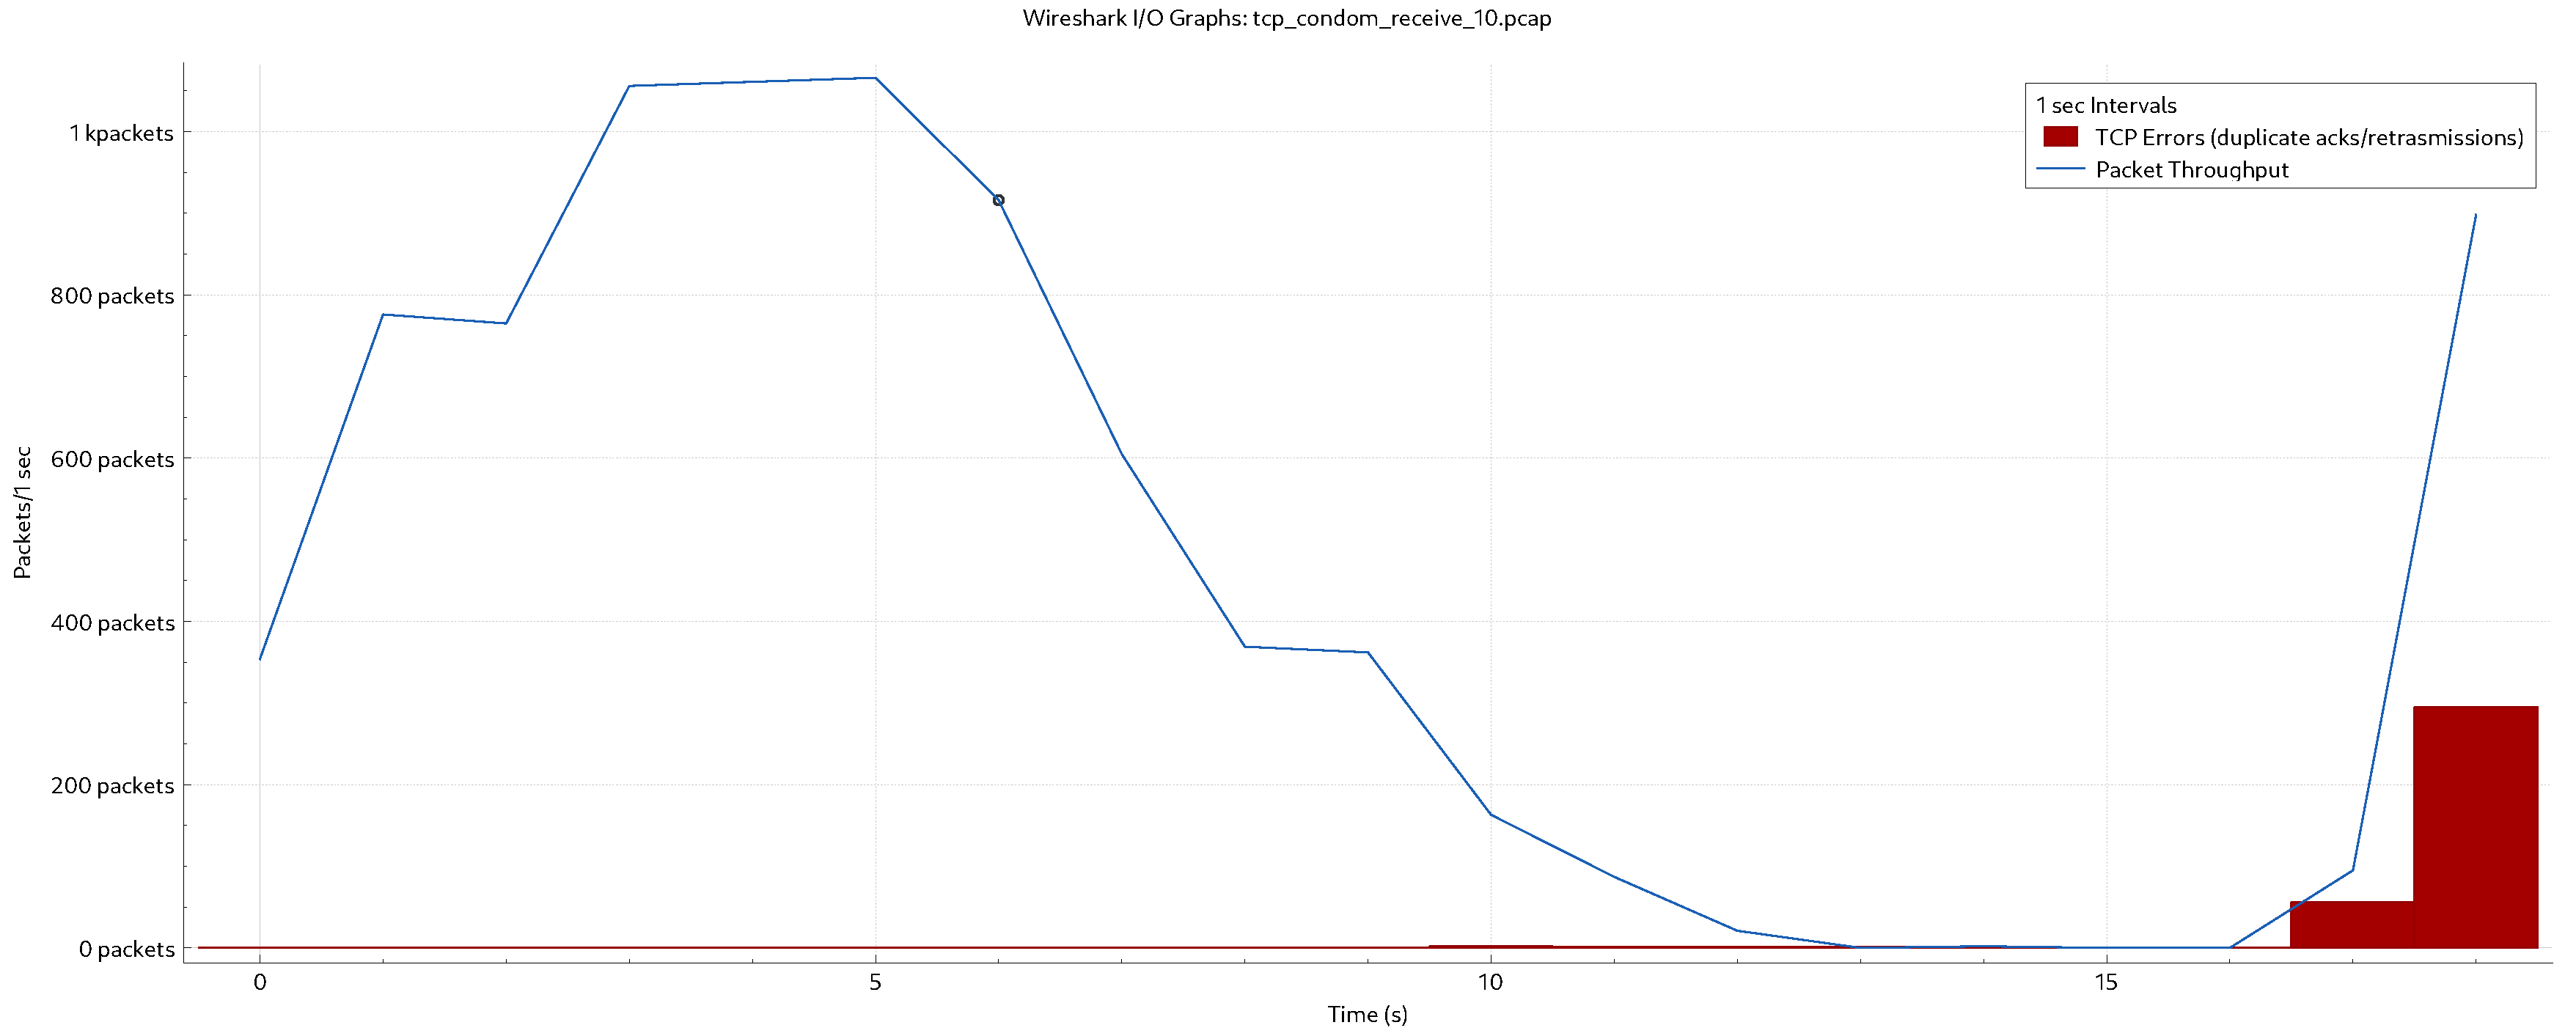
\includegraphics[width=0.75\linewidth]{images/PacketErrorsSaltWater.pdf}
    \caption{Packets/s (MA) on the receiver side + TCP errors, reverse flag set to True}
    \label{fig:enter-label}
\end{figure}

\onecolumn
\section{Python code}
\label{sec:python}

To run the various \texttt{iperf3} tests and collect aggregated results, we crafted a Python script with the following capabilities:

\begin{itemize}
    \item The script can autonomously run \texttt{iperf3} tests on a Linux machine.
    \item Every time a test, which is performed $N$ times, finishes, the script computes and prints out a table containing minimum, maximum, mean, median and standard deviation over the $N$ iterations.
    \item The various tests to run can be listed in a CSV file. Each CSV line specifies a name for the test, the number $N$ of iterations and additional parameters for the \texttt{iperf3} command (the protocol to use, the server's IP address, the desired bitrate etc.).
    \item Each time a single iteration of a test is executed, a PCAP file containing every packet sent or received during that iteration is saved in a folder named after the test.  
    For example, the test "realtek" with $N=5$ will generate five PCAPs:  
    \texttt{realtek\_1.pcap} to \texttt{realtek\_5.pcap}.
\end{itemize}

\hfill\\

\begin{minted}[fontsize=\small, breaklines]{python}
import subprocess
import time
import numpy as np
import csv

def run_iperf(name, server_ip, bind_ip, reverse, repetitions, pcap_fileNoExt, server_port, duration, udp, bitrate, app_buff_length):
    results = []
        
    try:
        for i in range(repetitions):
            # Start tcpdump to capture traffic
            tcpdump_process = subprocess.Popen(
                ["tcpdump", "-i", "any", "host", server_ip, "-w", pcap_fileNoExt+f"_{i+1}.pcap"],
                stdout=subprocess.DEVNULL, stderr=subprocess.DEVNULL
            )
            
            time.sleep(2)  # Allow tcpdump to start
            
            try:
                command = ["iperf3", "-c", server_ip, "-B", bind_ip, "-p", str(server_port), "-t", str(duration)]
                if reverse:
                    command.append("-R")
                if udp:
                    command.append("-u")
                if bitrate:
                    command.extend(["-b", str(bitrate)])
                if app_buff_length:
                    command.extend(["-l", str(app_buff_length)])
                
                result = subprocess.run(
                    command,
                    capture_output=True, text=True, check=True
                )
                
                for line in result.stdout.split("\n"):
                    if "receiver" in line:
                        parts = list(filter(None, line.split()))
                        if len(parts) > 6:
                            results.append(float(parts[6]))
            except subprocess.CalledProcessError as e:
                print(f"Error running iperf3: {e}")
            
            time.sleep(1)
            # Stop tcpdump
            tcpdump_process.terminate()
            tcpdump_process.wait()
    except Exception as e:
        print(e)

    return name, results

def compute_stats(name, data):
    if not data:
        print(f"No data collected for test {name}.")
        return name, None, None, None, None, None
    
    avg = np.mean(data)
    median = np.median(data)
    min_val = np.min(data)
    max_val = np.max(data)
    std_dev = np.std(data)
    
    print(f"Test: {name}")
    print(f"avg= {avg:.3f}")
    print(f"median= {median:.3f}")
    print(f"min= {min_val:.3f}")
    print(f"max= {max_val:.3f}")
    print(f"std= {std_dev:.3f}")
    
    return name, avg, median, min_val, max_val, std_dev

def read_csv_parameters(csv_file):
    tests = []
    with open(csv_file, mode='r') as file:
        reader = csv.reader(file)
        next(reader)  # Skip header
        for row in reader:
            name = row[0]
            server_ip = row[1]
            bind_ip = row[2]
            reverse = row[3].strip().lower() == 'true'
            repetitions = int(row[4])
            pcap_fileNoExt = row[5]
            server_port = int(row[6]) if len(row) > 6 else 5201  # Default port 5201
            duration = int(row[7]) if len(row) > 7 else 10  # Default 10s
            udp = row[8].strip().lower() == 'true' if len(row) > 8 else False
            bitrate = row[9] if len(row) > 9 and row[9] else None
            app_buff_length = row[10] if len(row) > 10 and row[10] else None
            
            tests.append((name, server_ip, bind_ip, reverse, repetitions, pcap_fileNoExt, server_port, duration, udp, bitrate, app_buff_length))
    return tests

def save_results_to_csv(results):
    for result in results:
        test_name = result[0]
        output_csv = f"{test_name}_results.csv"
        with open(output_csv, mode='w', newline='') as file:
            writer = csv.writer(file)
            writer.writerow(["Test Name", "Avg Throughput", "Median", "Min", "Max", "Std Dev"])
            writer.writerow(result)
        print(f"Results saved to {output_csv}")

if __name__ == "__main__":
    input_csv = "test_parameters.csv"  # Input CSV file
    
    test_cases = read_csv_parameters(input_csv)
    all_results = []
    
    for test in test_cases:
        print(f"Running test with parameters: {test}")
        name, throughput_data = run_iperf(*test)
        test_results = compute_stats(name, throughput_data)
        all_results.append(test_results)
    
    save_results_to_csv(all_results)
\end{minted}

\hfill\\
\hfill\\
An example of the CSV file is as follows:
% % First part (first 3 columns)
% \begin{table}[htbp]
% \centering
% \begin{tabularx}{\columnwidth}{|X|X|X|}
% \hline
% \textbf{name} & \textbf{server\_ip} & \textbf{bind\_ip} \\
% \hline
% TCP\_send & 192.168.1.74 & 192.168.1.136 \\
% TCP\_receive & 192.168.1.74 & 192.168.1.136 \\
% \hline
% \end{tabularx}
% \end{table}

% % Second part (next 3 columns)
% \begin{table}[htbp]
% \centering
% \begin{tabularx}{\columnwidth}{|X|X|X|}
% \hline
% \textbf{reverse} & \textbf{repetitions} & \textbf{pcap\_file\_noExt} \\
% \hline
% FALSE & 10 & send \\
% TRUE & 10 & receive \\
% \hline
% \end{tabularx}
% \end{table}

% % Third part (next 3 columns)
% \begin{table}[htbp]
% \centering
% \begin{tabularx}{\columnwidth}{|X|X|X|}
% \hline
% \textbf{server\_port} & \textbf{duration} & \textbf{udp} \\
% \hline
% 5202 & 10 &  \\
% 5202 & 10 &  \\
% \hline
% \end{tabularx}
% \end{table}

% % Fourth part (last 2 columns)
% \begin{table}[htbp]
% \centering
% \begin{tabularx}{\columnwidth}{|X|X|}
% \hline
% \textbf{bitrate} & \textbf{app\_buff\_length} \\
% \hline
%  &  \\
%  &  \\
% \hline
% \end{tabularx}
% \end{table}


\begin{table}[htbp]
\centering
\begin{tabularx}{\textwidth}{|X|X|X|X|}
\hline
\textbf{name} & \textbf{server\_ip} & \textbf{bind\_ip} & \textbf{reverse} \\
\hline
TCP\_send & 192.168.1.74 & 192.168.1.136 & False \\
TCP\_receive & 192.168.1.74 & 192.168.1.136 & True \\
\hline
\end{tabularx}
\end{table}

\begin{table}[htbp]
\centering
\begin{tabularx}{\textwidth}{|X|X|X|X|}
\hline
\textbf{repetitions} & \textbf{pcap\_file\_noExt} & \textbf{server\_port} & \textbf{duration} \\
\hline
10 & send & 5202 & 10 \\
10 & receive & 5202 & 10 \\
\hline
\end{tabularx}
\end{table}


\begin{table}[htbp]
\centering
\begin{tabularx}{\textwidth}{|X|X|X|}
\hline
\textbf{udp} & \textbf{bitrate} & \textbf{app\_buff\_length} \\
\hline
 &  & \\
 &  & \\
\hline
\end{tabularx}
\end{table}
